% =============================================================================
% EXPERIMENTO CONTROLADO (14:25 a 14:50)   [Script 02 | Exercício 1]
% =============================================================================
\section[Experimento]{Experimento controlado}

\begin{frame}{O ``padrão ouro'': a aleatorização}
  \centering
  \begin{tikzpicture}[scale=0.8,every node/.style={transform shape}]
    \node[cx,minimum width=2.4cm] (pop) at (0,0) {Elegíveis};
    \node[cxi,minimum width=2.2cm,font=\footnotesize\bfseries] (sorteio) at (3.2,0) {Sorteio};
    \node[cxl,minimum width=2.4cm] (trat) at (6.6,1.0) {\textbf{Tratamento}};
    \node[cxi,minimum width=2.4cm] (ctrl) at (6.6,-1.0) {\textbf{Controle}};
    \node[cxl,minimum width=2.2cm,font=\footnotesize\bfseries] (imp) at (10.2,0) {Impacto\\$=\bar Y_T-\bar Y_C$};
    \draw[seta] (pop) -- (sorteio);
    \draw[seta] (sorteio) -- (trat); \draw[seta] (sorteio) -- (ctrl);
    \draw[seta] (trat) -- (imp); \draw[seta] (ctrl) -- (imp);
  \end{tikzpicture}
  \vspace{0.2cm}
  \begin{itemize}
    \item O sorteio torna os grupos equivalentes \destaque{em média}, nas características observadas e \textbf{não observadas};
    \item Só difere o receber ou não a política: a diferença nos resultados é o \ind{impacto}.
  \end{itemize}
\end{frame}

\begin{frame}{Experimento: características e exemplos}
  \carac{grupo de \textbf{controle sorteado}}
        {sorteio bem executado; sem contaminação (\emph{spillovers}); atrito não seletivo}
        {efeito médio (ATE); ITT se a adesão é imperfeita}
        {desenho \textbf{antes} da política; amostra com poder estatístico}
        {recursos escassos, pilotos, expansão em fases}
  \vspace{0.15cm}
  \textbf{\footnotesize\color{azul}Exemplos em políticas públicas}\par
    \scriptsize
    \begin{itemize}
      \item \textbf{Quênia:} desparasitação em escolas, entrada sorteada por fases; mais frequência escolar (Miguel e Kremer, 2004).
      \item \textbf{México:} Progresa, localidades sorteadas para entrar primeiro (Gertler, 2004; Schultz, 2004); Seguro Popular, gastos com saúde caíram 23\% (King et al., 2009).
      \item \textbf{Hipotético (nosso Qualifica):} sorteio das vagas excedentes de um curso de qualificação municipal.
    \end{itemize}
  
\end{frame}

\begin{frame}{Por que funciona? Os grupos ficam equilibrados}
  \centering
  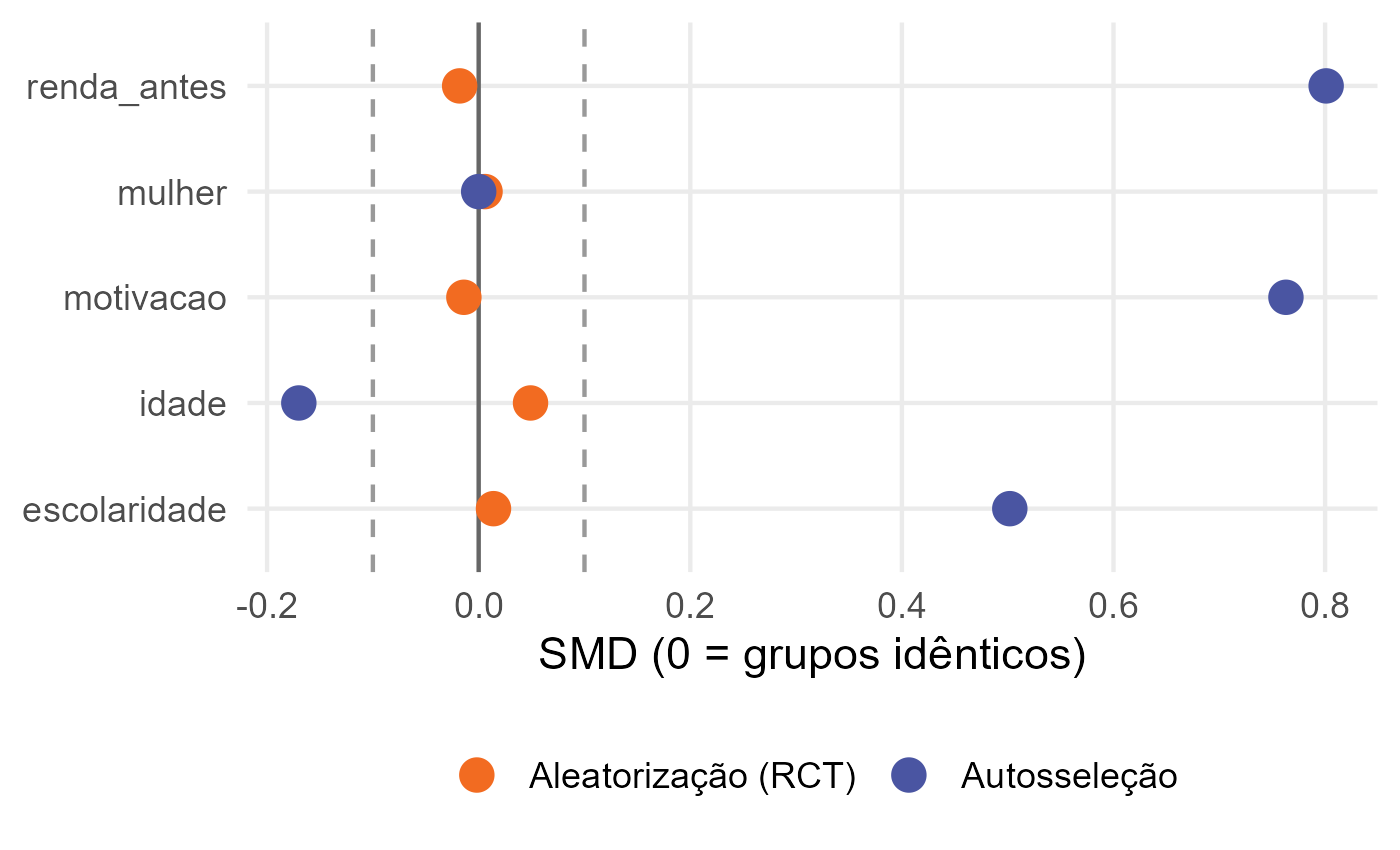
\includegraphics[height=4.4cm]{02_balanco.png}\par
  \footnotesize Com sorteio, até a \ind{motivação} (não observada) fica equilibrada. SMD: diferença padronizada de médias.
\end{frame}

\begin{frame}{Mil avaliações, dois métodos (Monte Carlo)}
  \centering
  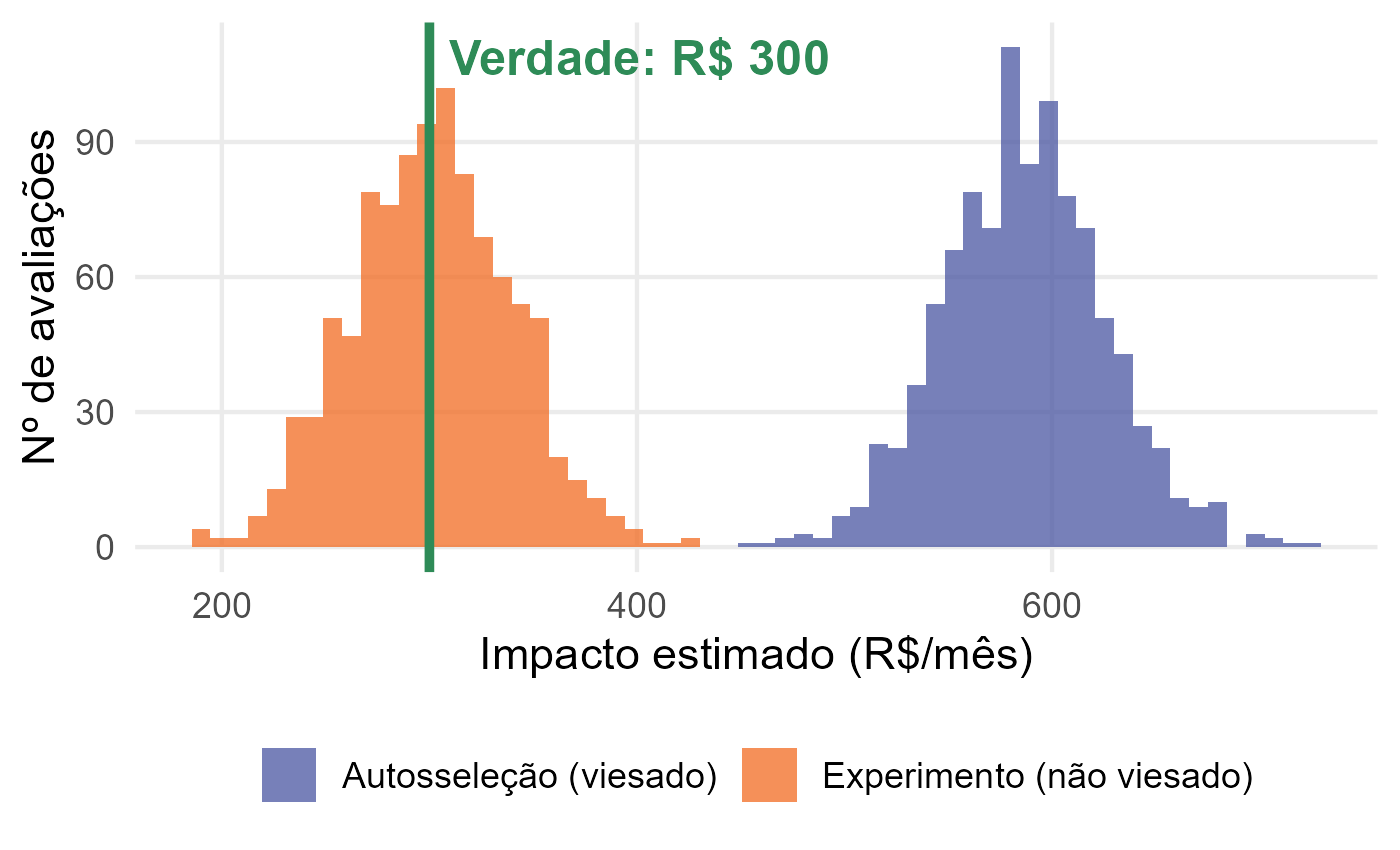
\includegraphics[height=4.3cm]{02_montecarlo.png}\par
  \footnotesize O sorteio acerta \emph{em média} (301); a autosseleção erra \alert{sempre para o mesmo lado} (587). Verdade: 300.
\end{frame}

\begin{frame}{Passo a passo: experimento (1 de 2)}
  \relax{\scriptsize\setlength{\tabcolsep}{2.5pt}\renewcommand{\arraystretch}{1.1}\begin{tabular}{@{}cP{2.55cm}P{2.75cm}P{3.6cm}@{}}
    \toprule
    \cabecalho{Como ler e decidir}
    \linha{1}{Compare tratados e controles \textbf{antes} do programa (SMD)}{idade 0,05\newline mulher 0,01\newline escolaridade 0,01\newline renda antes $-0{,}02$}{Todos $|\text{SMD}|<0{,}10$: o sorteio equilibrou os grupos. \textbf{Siga.} Se não, revise o sorteio.}
    \linha{2}{Estime o efeito: diferença de médias (\cod{t.test}) ou regressão}{efeito = 295,2\newline EP = 11,4\newline IC 95\%: 273 a 318}{Participantes ganham ${\approx}$ R\$ 295 a mais. O IC não inclui zero: efeito \textbf{significativo}.}
    \ultimalinha{3}{Reestime com covariáveis (só para ganhar precisão)}{efeito = 302,1\newline EP = 3,4}{Mesma magnitude, EP três vezes menor. O viés já estava resolvido pelo sorteio.}
  \end{tabular}}
  \caixaconclusao{o Qualifica aumenta a renda em cerca de R\$ 300 (IC 273 a 318). Dados simulados do script 02.}
\end{frame}

\begin{frame}{Passo a passo: experimento (2 de 2)}
  \relax{\scriptsize\setlength{\tabcolsep}{2.5pt}\renewcommand{\arraystretch}{1.1}\begin{tabular}{@{}cP{2.55cm}P{2.75cm}P{3.6cm}@{}}
    \toprule
    \cabecalho{Como ler e decidir}
    \linha{4}{Cheque a \textbf{adesão} (\emph{compliance})}{adesão de 70\%\newline ITT = 193\newline efeito sobre aderentes = 293}{Relate o \textbf{ITT} (efeito da \emph{oferta}) e o efeito sobre quem aderiu.}
    \linha{5}{Cheque o \textbf{atrito}}{3,6\% saíram\newline se saem só os piores: 345}{Compare quem saiu em cada grupo. Atrito seletivo faz o viés voltar.}
    \ultimalinha{6}{Confira o \textbf{poder} (\cod{power.t.test})}{R\$ 300: 34 por grupo\newline R\$ 100: 291 por grupo}{Efeitos pequenos exigem amostras grandes. Calcule \textbf{antes} do experimento.}
  \end{tabular}}
  \caixaconclusao{adesão incompleta e atrito mudam \emph{o que} o número significa.}
\end{frame}

\begin{frame}{Exercício 1: viés de seleção e sorteio (12 min)}
  \begin{exerciciobox}{\texttt{atividades/exercicio\_01\_vies\_e\_experimento.R}}
    \small
    \begin{enumerate}
      \item Varie a força da motivação (0 a 1,5): compare o viés da \textbf{comparação ingênua} com o do \textbf{sorteio};
      \item Quantas pessoas por grupo para detectar R\$ 100 com poder de 90\%?
    \end{enumerate}
  \end{exerciciobox}
  \vspace{0.2cm}
  \textbf{Discutam:} por que o sorteio recupera ${\approx}$ R\$ 300 mesmo quando a motivação pesa muito na inscrição?
\end{frame}
